\documentclass[11pt,a4paper]{article}
\usepackage[T1]{fontenc}\usepackage[utf8]{inputenc}\usepackage[scaled=0.95]{helvet}\renewcommand{\familydefault}{\sfdefault}
\usepackage[a4paper,margin=2.2cm]{geometry}\usepackage{graphicx,booktabs,longtable,amsmath,caption,xcolor,enumitem,array,float}\usepackage[hidelinks]{hyperref}
\captionsetup{font=small,labelfont=bf}\setlength{\parskip}{0.55em}\setlength{\parindent}{0pt}\setlist{itemsep=0.25em,topsep=0.3em}\widowpenalty=10000\clubpenalty=10000\raggedbottom
\newcommand{\docversion}{2026-11-11-10-52-13}
\begin{document}
{\LARGE\bfseries Automobiles and curb along rue de Terrebonne\par}\vspace{0.3em}
{\large Registered vehicles known by postal district, modelled below it; legal curb measured block face by block face\par}\vspace{0.6em}
Rick Hoge, PhD \hfill November 11, 2026 \hfill version \docversion
\begin{center}\colorbox{red!15}{\parbox{0.96\textwidth}{\centering\textbf{\textcolor{red!70!black}{DRAFT for the author\textquoteright{}s review, November 11, 2026. Not yet checked line by line; figures may change.}}}}\end{center}
\section*{Lay summary}
How many cars belong to the households along the Terrebonne bike lane, and how much curb is there to park them? Québec\textquoteright{}s vehicle registry, as released, places each vehicle only in a postal district of about 10,000 households (H4A or H4B), not on a street. This note goes one step finer, and says which parts are measured and which are estimated.

Measured: the curb. Using the City\textquoteright{}s inventory of parking signs, every side of every block was read for stretches where parking is forbidden at all times. The 22 census areas that touch the lane, reaching about one block to each side, hold 37 km of legal curb. That is an upper limit: driveways, hydrants and bus stops are not removed.

Estimated: the cars. Census facts about each small area (renters, commuters who drive, household size, income) were used to share out each district\textquoteright{}s registered automobiles. For the corridor\textquoteright{}s 5,471 households the estimate is about 4,600 automobiles, between 4,400 and 4,900: 0.84 per household. For a single small area the estimate is uncertain by about a quarter either way.

The method was tested where the answer is known. Sharing a group of districts\textquoteright{} total among its members, it was off by 5 per cent at the median, against 14 per cent for a simple split by number of households.

At 5.5 m per car, the corridor\textquoteright{}s legal curb would hold about 6,800 cars, more than the estimated number registered there. This is not a measure of parking difficulty: it ignores garages and driveways, which about 70 per cent of dwellings on Terrebonne have, as well as visitors, time limits and where on the block a space is. A count of cars seen on a 2015 night agrees with the estimate only in order of magnitude.

The note makes no recommendation.

\begin{figure}[H]\centering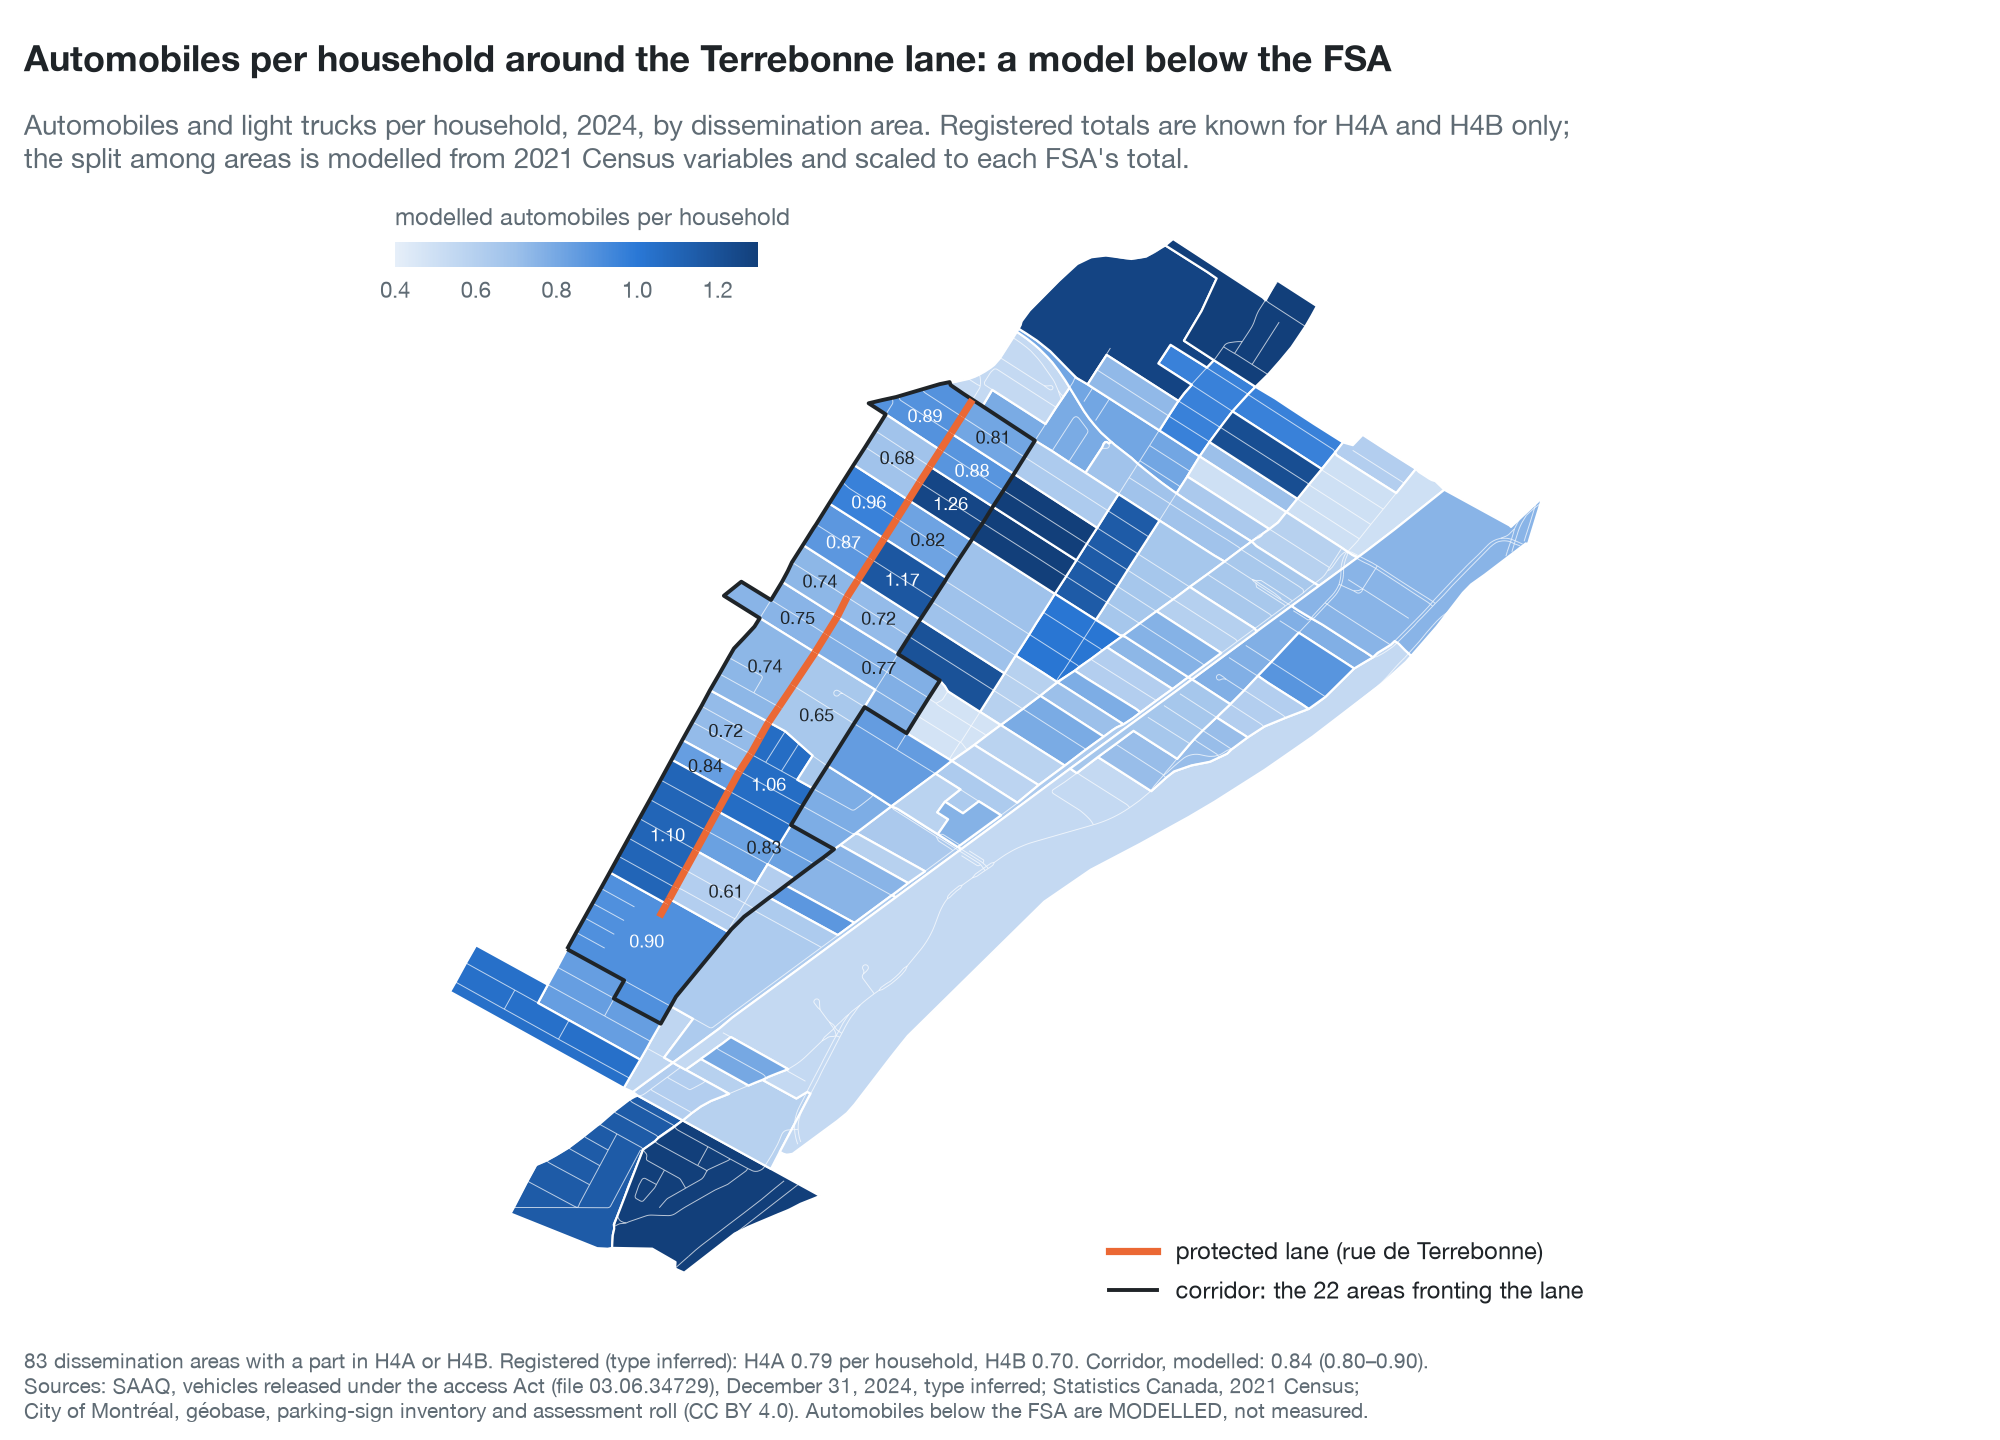
\includegraphics[width=1.0\textwidth]{../derived/figures/overview-map/overview_map_en.png}\caption{Overview. Modelled automobiles and light trucks per household by dissemination area, 2024. The registered totals are known for the two FSAs only; the split among areas is a model.}\end{figure}

\tableofcontents
\newpage
\section{Question}
The vehicle files the SAAQ released under the access Act for 2023 and 2024 (file 03.06.34729) locate each vehicle to its forward sortation area (FSA, the first three characters of the postal code), and no finer. The protected bike lane on rue de Terrebonne lies in two FSAs: H4B west of avenue Royal, H4A east of it. On December 31, 2024 they held 7{,}351 and 9{,}598 automobiles and light trucks (type inferred from make, model and model year, as in the note of the repository \emph{Quebec-vehicle-registrations}), that is 0.70 and 0.79 per household of the 2021 Census.

An FSA holds ten to twelve thousand households; the lane's surroundings are a fraction of each. This note asks what can be said at a finer grain, about the dissemination areas that front the lane: how many automobiles are registered there, and how much legal curb they hold. The two halves of the answer are of different kinds, and the note keeps them apart throughout:
\begin{itemize}
\item \textbf{Curb is measured}, block face by block face, from the City\textquoteright{}s géobase and its inventory of parking signs.
\item \textbf{Automobiles below the FSA are modelled}, from 2021 Census variables, and scaled so that the areas of each FSA sum to its registered total. Within an FSA the split is an estimate with an interval, never a count.
\end{itemize}
The 2015 LiDAR and the aerial imagery read for the 1954--55 plans work serve as a check, not as an input. The note makes no recommendation.

\section{Data}
\begin{itemize}
\item \textbf{Vehicles.} SAAQ, files released under the access Act for December 31, 2023 and 2024, by FSA; the table \texttt{type\_by\_fsa.csv} of \emph{Quebec-vehicle-registrations} (type inferred; all automobiles and light trucks, whether registered to a person or to a business: the release carries no class).
\item \textbf{Census.} Statistics Canada, 2021 Census profile by FSA (98-401-X2021013) and by dissemination area (98-401-X2021006), and the dissemination-area boundaries. Counts are randomly rounded to 5 by Statistics Canada; tenure, commuting and income come from the 25\,\% sample.
\item \textbf{Curb.} City of Montréal, géobase (street segments, October 14, 2026) and \emph{Signalisation -- stationnement} (sign inventory, October 23, 2026), both CC BY 4.0.
\item \textbf{Dwellings.} City of Montréal, \emph{Unités d\textquoteright{}évaluation foncière} (assessment roll, CC BY 4.0), used to share a dissemination area that straddles two FSAs and to count the dwellings addressed on rue de Terrebonne; FSA polygons from DMTI Spatial, CanMap Postal Code Suite v2024.3 (under licence, not redistributed).
\item \textbf{Checks.} The cars counted by eye on the City\textquoteright{}s 2015 night LiDAR and the garage and driveway readings, from the folder \emph{1954-underwriters-plans-terrebonne-garages}; the parking counts of the borough\textquoteright{}s 2023 study (EXP), as transcribed in \emph{2026-parking-supply-demand-survey-context}.
\end{itemize}

\section{Method}
\subsection{Dissemination areas and FSAs}
Dissemination areas do not nest in FSAs. Each area is shared among FSAs in proportion to the dwellings of the assessment roll found in each FSA polygon. Rebuilt this way from dissemination areas, the households of the island\textquoteright{}s 96 FSAs of 1{,}000 households or more differ from Statistics Canada\textquoteright{}s own FSA profile by 0.5\,\% at the median (H4A $-$1.2\,\%, H4B $-$1.2\,\%). 83 areas have a part in H4A or H4B.

\subsection{The corridor}
The corridor is the set of 22 dissemination areas that hold a block face of rue de Terrebonne along the lane, from its west end to Girouard. They reach about one block to each side (Somerled is about 260\,m north of the lane, Monkland about 285\,m south); 17 of them have nine-tenths or more of their surface within 300\,m of the lane (the others are the larger areas toward the west end, the smallest share being 19\,\%), and no area outside the set has half its surface within that distance.

\subsection{Legal curb}
A block face is one side of one géobase segment (autoroutes, bridges, tunnels and back lanes left out). A segment runs from the centre of one intersection to the centre of the next. A face\textquoteright{}s legal curb is its length, less 10\,m at each end, less the stretches where a sign forbids stopping or parking at all times («\,\textbackslash A EN TOUT TEMPS\,», «\,\textbackslash P EN TOUT TEMPS\,»). The stretch a sign governs runs from its pole to the next pole in the direction of its arrow; a sign without an arrow governs the stretches on both sides of its pole. Where the usual reading of the arrows leaves a stretch claimed both by an all-time prohibition and by another parking rule (hours, days, a time limit: a rule that implies parking exists there), the other reading is taken for that face if it leaves fewer such stretches; a stretch still claimed both ways counts for half.

The 10\,m at each end is the half roadway of the cross street (5\,m, an assumption: the local cross streets measure 9.0 to 9.4\,m from curb to curb on the 2015 LiDAR, rue de Terrebonne 11.0\,m) plus the 5\,m next to an intersection where the Highway Safety Code forbids stopping, signed or not (art.~386, par.~4).

The result is an \textbf{upper bound} on legal curb: driveways, hydrants, bus stops, hourly rules, permit zones and seasonal rules are not deducted. Places are legal curb divided by 5, 5.5 and 6\,m.

\textbf{Check on rue de Terrebonne}, where the layout is known: the reading finds parking on the south side west of Cavendish and on the north side east of it, one band, as built in 2024: 1{,}306\,m of legal curb, 238 places at 5.5\,m. The borough\textquoteright{}s 2023 study counted 478 places on the two sides before the lane (report p.~40): 230 westbound and 248 eastbound.

\subsection{Automobiles below the FSA}
\begin{enumerate}
\item Across the 114 FSAs beginning with H that hold 1{,}000 households or more, the logarithm of automobiles per household is regressed on four census variables: the share of renter households, the share of commuters who drive, persons per household, and the logarithm of the median household income. The regression is robust (Huber weights), because a few FSAs hold fleets registered to businesses (H2Y, H2Z, H3A, H3B, H4P, H9P: registered counts more than 1.5 times what their census variables predict).
\item The rate of each dissemination area is predicted from its own census variables.
\item The predictions are scaled so that the parts of the areas lying in each FSA sum to that FSA\textquoteright{}s registered total. The scale factors of H4A and H4B are 1.07 and 0.99.
\end{enumerate}
Specifications were compared by leaving each FSA out in turn (Table~\ref{tab:spec}); the one used has the smallest error at the 90th percentile and close to the smallest at the median. Dwelling type adds nothing once tenure, commuting and household size are in.

\textbf{Intervals} come from 2{,}000 draws, each combining: the FSAs resampled and the model refitted; the sampling error of the 25\,\% sample variables in each dissemination area; an unexplained factor for each area, whose spread is the one measured by the downscaling test below; and the scaling to the FSA totals. Dissemination areas are about twenty times smaller than FSAs, and their true unexplained spread may be larger than the one measured among FSAs: the tables also carry intervals with that spread doubled, which are wider by a few points only, because the sampling error of the census variables dominates. The intervals do not cover what the model cannot see: the vehicles are those of December 31, 2024 and the census is of May 2021; the type is inferred; vehicles registered to businesses are in the totals.

\section{Results}
\subsection{Does the model work where the answer is known?}
Two tests, both at the level of FSAs, the only level at which registered counts exist.

\emph{Each FSA left out in turn.} The model fitted on the other FSAs predicts the left-out FSA\textquoteright{}s rate within 5.4\,\% at the median (24\,\% at the 90th percentile, the business FSAs included). H4A is under-predicted by 11\,\%, H4B by 0.6\,\%.

\emph{Downscaling, one level up.} Neighbouring FSAs were grouped by threes (27 groups, 103 FSAs); for each group the model was fitted without its members, and the group\textquoteright{}s registered total was shared among them by the model. This is the operation the note performs below the FSA, done where it can be checked. The share of each FSA is off by 4.6\,\% at the median (26\,\% at the 90th percentile); sharing in proportion to households is off by 13.9\,\% (42\,\%). Without the groups that hold a business FSA: 3.9\,\% against 12.3\,\%. For H4A and H4B taken as one group, the model\textquoteright{}s shares are off by $-$4.6\,\% and +6.0\,\%, the household split by $-$5.5\,\% and +7.1\,\%: for this pair the model gains little.

\begin{figure}[H]\centering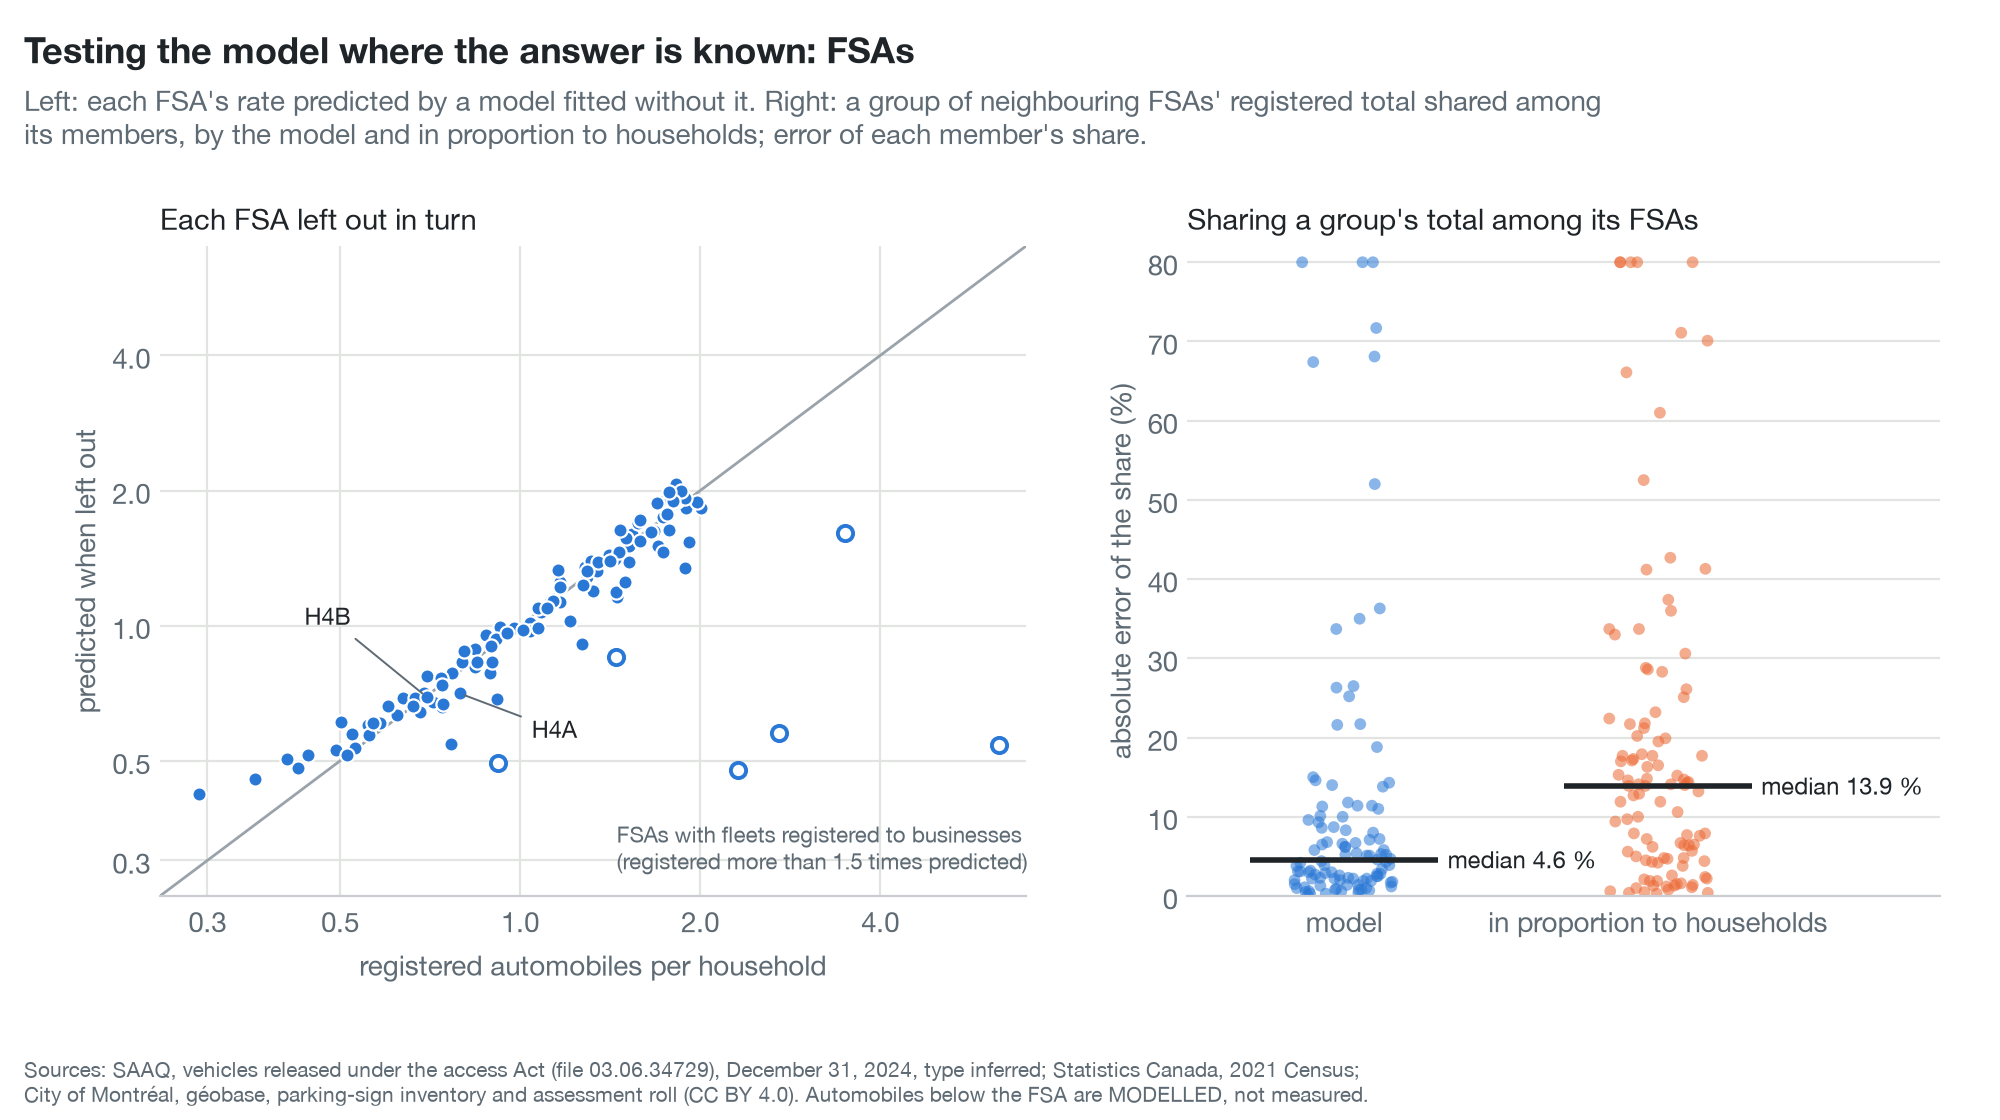
\includegraphics[width=1.0\textwidth]{../derived/figures/model-tests/model_tests_en.png}\caption{The two tests. Left: each FSA\textquoteright{}s rate predicted without it (hollow: FSAs with fleets). Right: error of each FSA\textquoteright{}s share of its group\textquoteright{}s total; errors above 80\,\% drawn at 80.}\end{figure}

The tests say the model shares a total among FSAs better than households alone do. They cannot say how well it shares an FSA among its dissemination areas: no registered count exists at that level.

\subsection{The corridor}
\begin{table}[H]\centering\small
\caption{Modelled automobiles and measured legal curb. Interval: 90\,\%. Places: legal curb at 6\,m to 5\,m per vehicle (upper bound). Last column: modelled automobiles per place at 5.5\,m.}\label{tab:sets}
\footnotesize\setlength{\tabcolsep}{4pt}\begin{tabular}{@{}p{3.3cm}rrrrrrrr@{}}\toprule
 & areas & hh. & autos & interval & per hh. & curb km & places & per place \\\midrule
Corridor & 22 & 5{,}471 & 4{,}622 & 4{,}382--4{,}927 & 0.84 & 37.2 & 6{,}192--7{,}431 & 0.68 \\
Other areas of H4A, H4B & 61 & 18{,}978 & 14{,}363 & 14{,}033--14{,}641 & 0.76 & 109.3 & 18{,}210--21{,}852 & 0.72 \\
All & 83 & 24{,}449 & 18{,}985 & 18{,}830--19{,}163 & 0.78 & 146.4 & 24{,}402--29{,}283 & 0.71 \\
\bottomrule\end{tabular}\end{table}
The corridor\textquoteright{}s 5{,}471 households are estimated to have 4{,}622 automobiles and light trucks registered (4{,}382 to 4{,}927), 0.84 per household (0.80 to 0.90); the other areas of the two FSAs, 0.76. The two alternative specifications give 4{,}616 and 4{,}683 for the corridor. Area by area the estimates run from 0.61 to 1.26 per household, and the 90\,\% interval of a single area is about 29\,\% of its estimate either way (Figure~\ref{fig:areas}, Table~\ref{tab:da}). The differences between neighbouring areas are mostly within those intervals.

\begin{figure}[H]\centering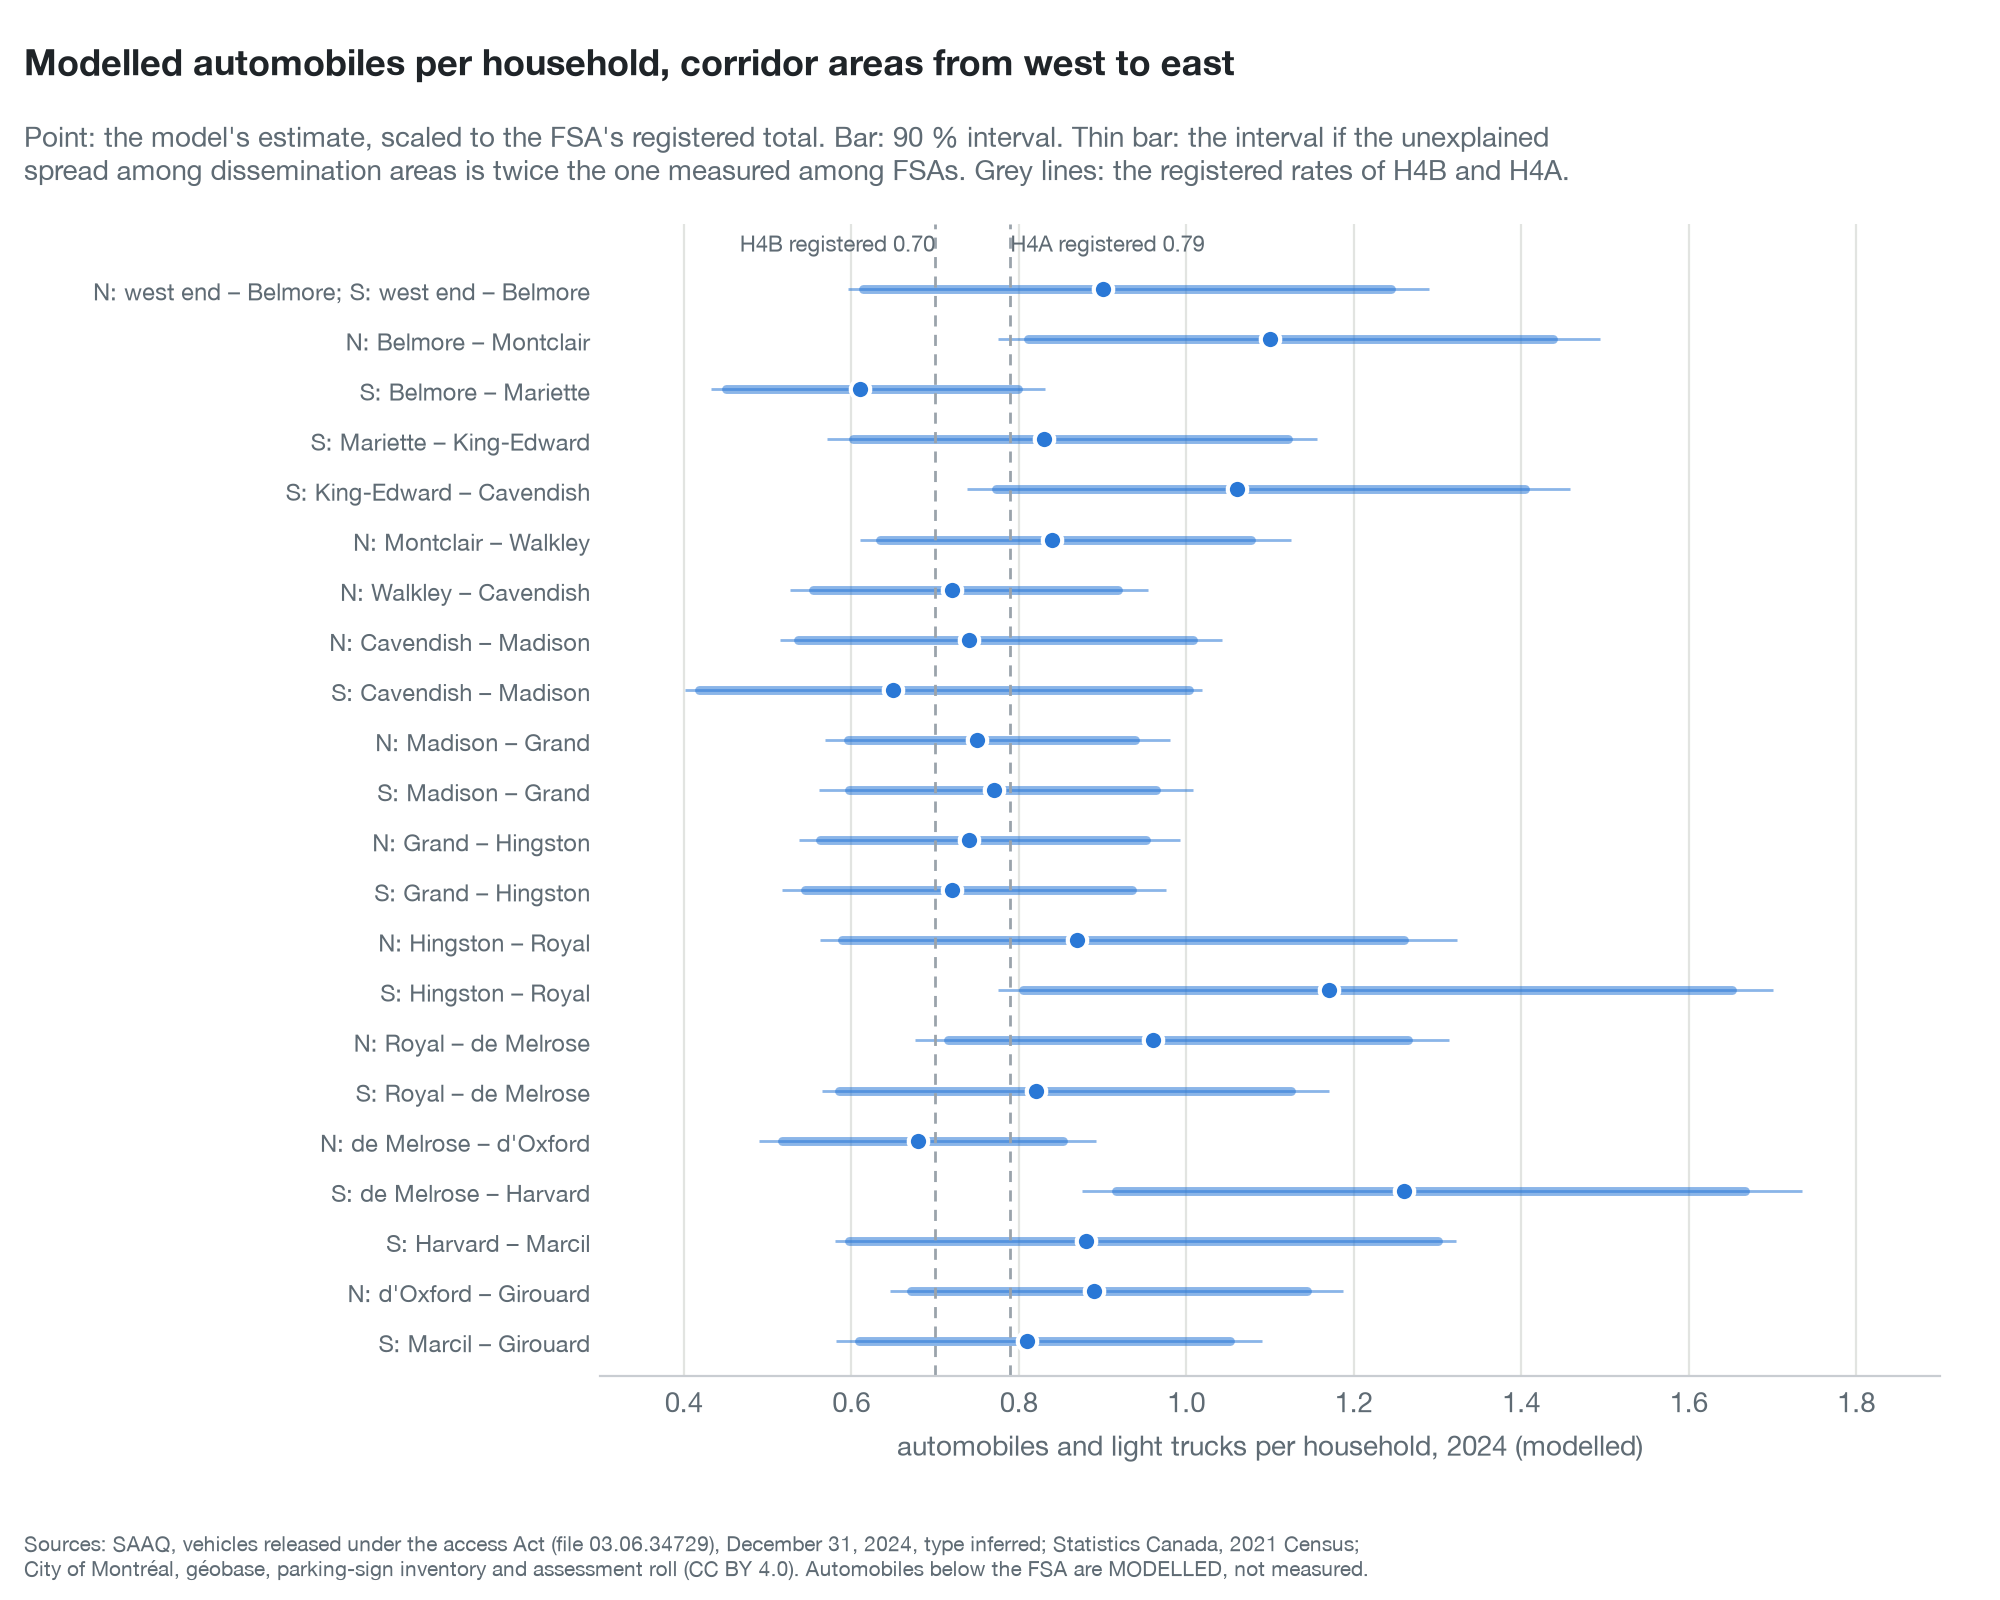
\includegraphics[width=\textwidth]{../derived/figures/area-estimates/area_estimates_en.png}\caption{Modelled automobiles per household, the corridor\textquoteright{}s areas from west to east.}\label{fig:areas}\end{figure}

\subsection{Legal curb}
The corridor holds 46.8\,km of curb; net of 10\,m at each end of each face, 8\,\% is forbidden at all times, leaving 37.2\,km of legal curb: 6{,}192 to 7{,}431 places at 6 to 5\,m, an upper bound. That is 6.8\,m of legal curb per household (5.8\,m in the other areas of the two FSAs).

\begin{figure}[H]\centering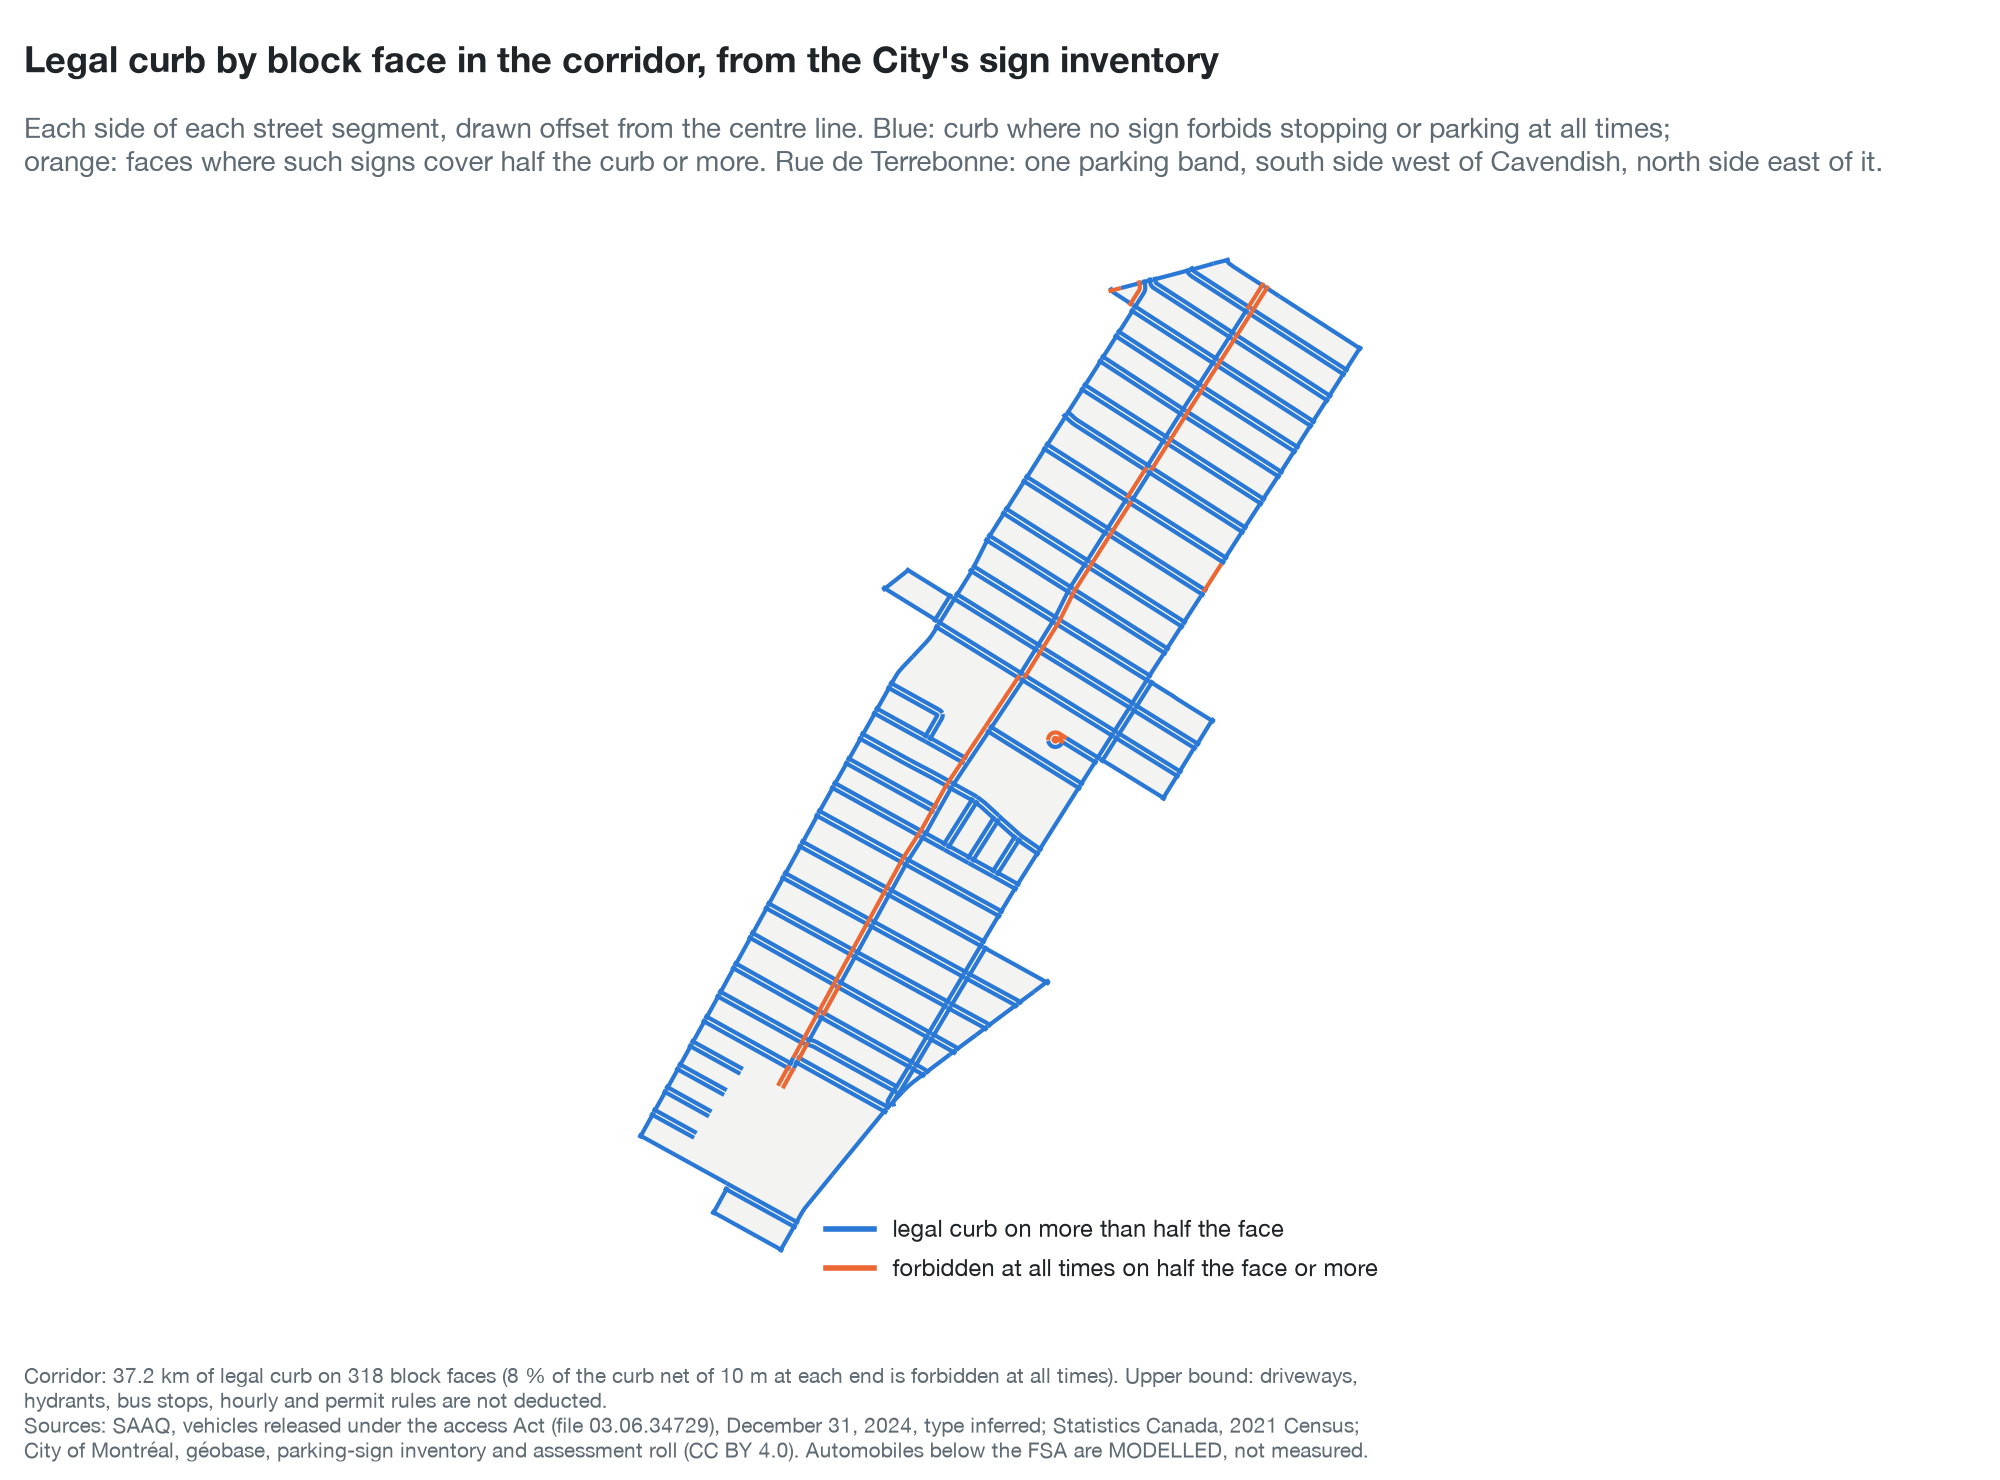
\includegraphics[width=0.92\textwidth]{../derived/figures/curb-map/curb_map_en.png}\caption{Block faces of the corridor. A face is drawn orange when all-time prohibitions cover half of it or more.}\end{figure}

\subsection{Automobiles beside curb}
At 5.5\,m per place the corridor has 0.68 modelled automobile per place of legal curb (0.65 to 0.73); in 5 of the 22 areas the estimate exceeds the area\textquoteright{}s own places (Figure~\ref{fig:both}).

\textbf{This ratio is not a measure of parking pressure, in either direction.} The curb figure is an upper bound (no driveway, hydrant or bus stop deducted, no hourly or permit rule). The automobile figure is every vehicle registered, wherever it is kept: off-street parking is in neither term, and on rue de Terrebonne itself 70\,\% of dwellings are in a building with a garage as built or a driveway today (188 of 268; \emph{1954-underwriters-plans-terrebonne-garages}). Visitors, institutions and vehicles from elsewhere use the same curb; a place at the far end of an area is not a place at one\textquoteright{}s door. The measurements of occupancy that exist are those of the borough\textquoteright{}s 2023 study: on Thursday, September 29, 2022, at 18:30--19:30, 247 cars on rue de Terrebonne\textquoteright{}s places (50\,\%) and 311 on the cross-street stubs (51\,\%) (EXP, Tables 3-2 and 3-3, as transcribed in \emph{2026-parking-supply-demand-survey-context}).

\begin{figure}[H]\centering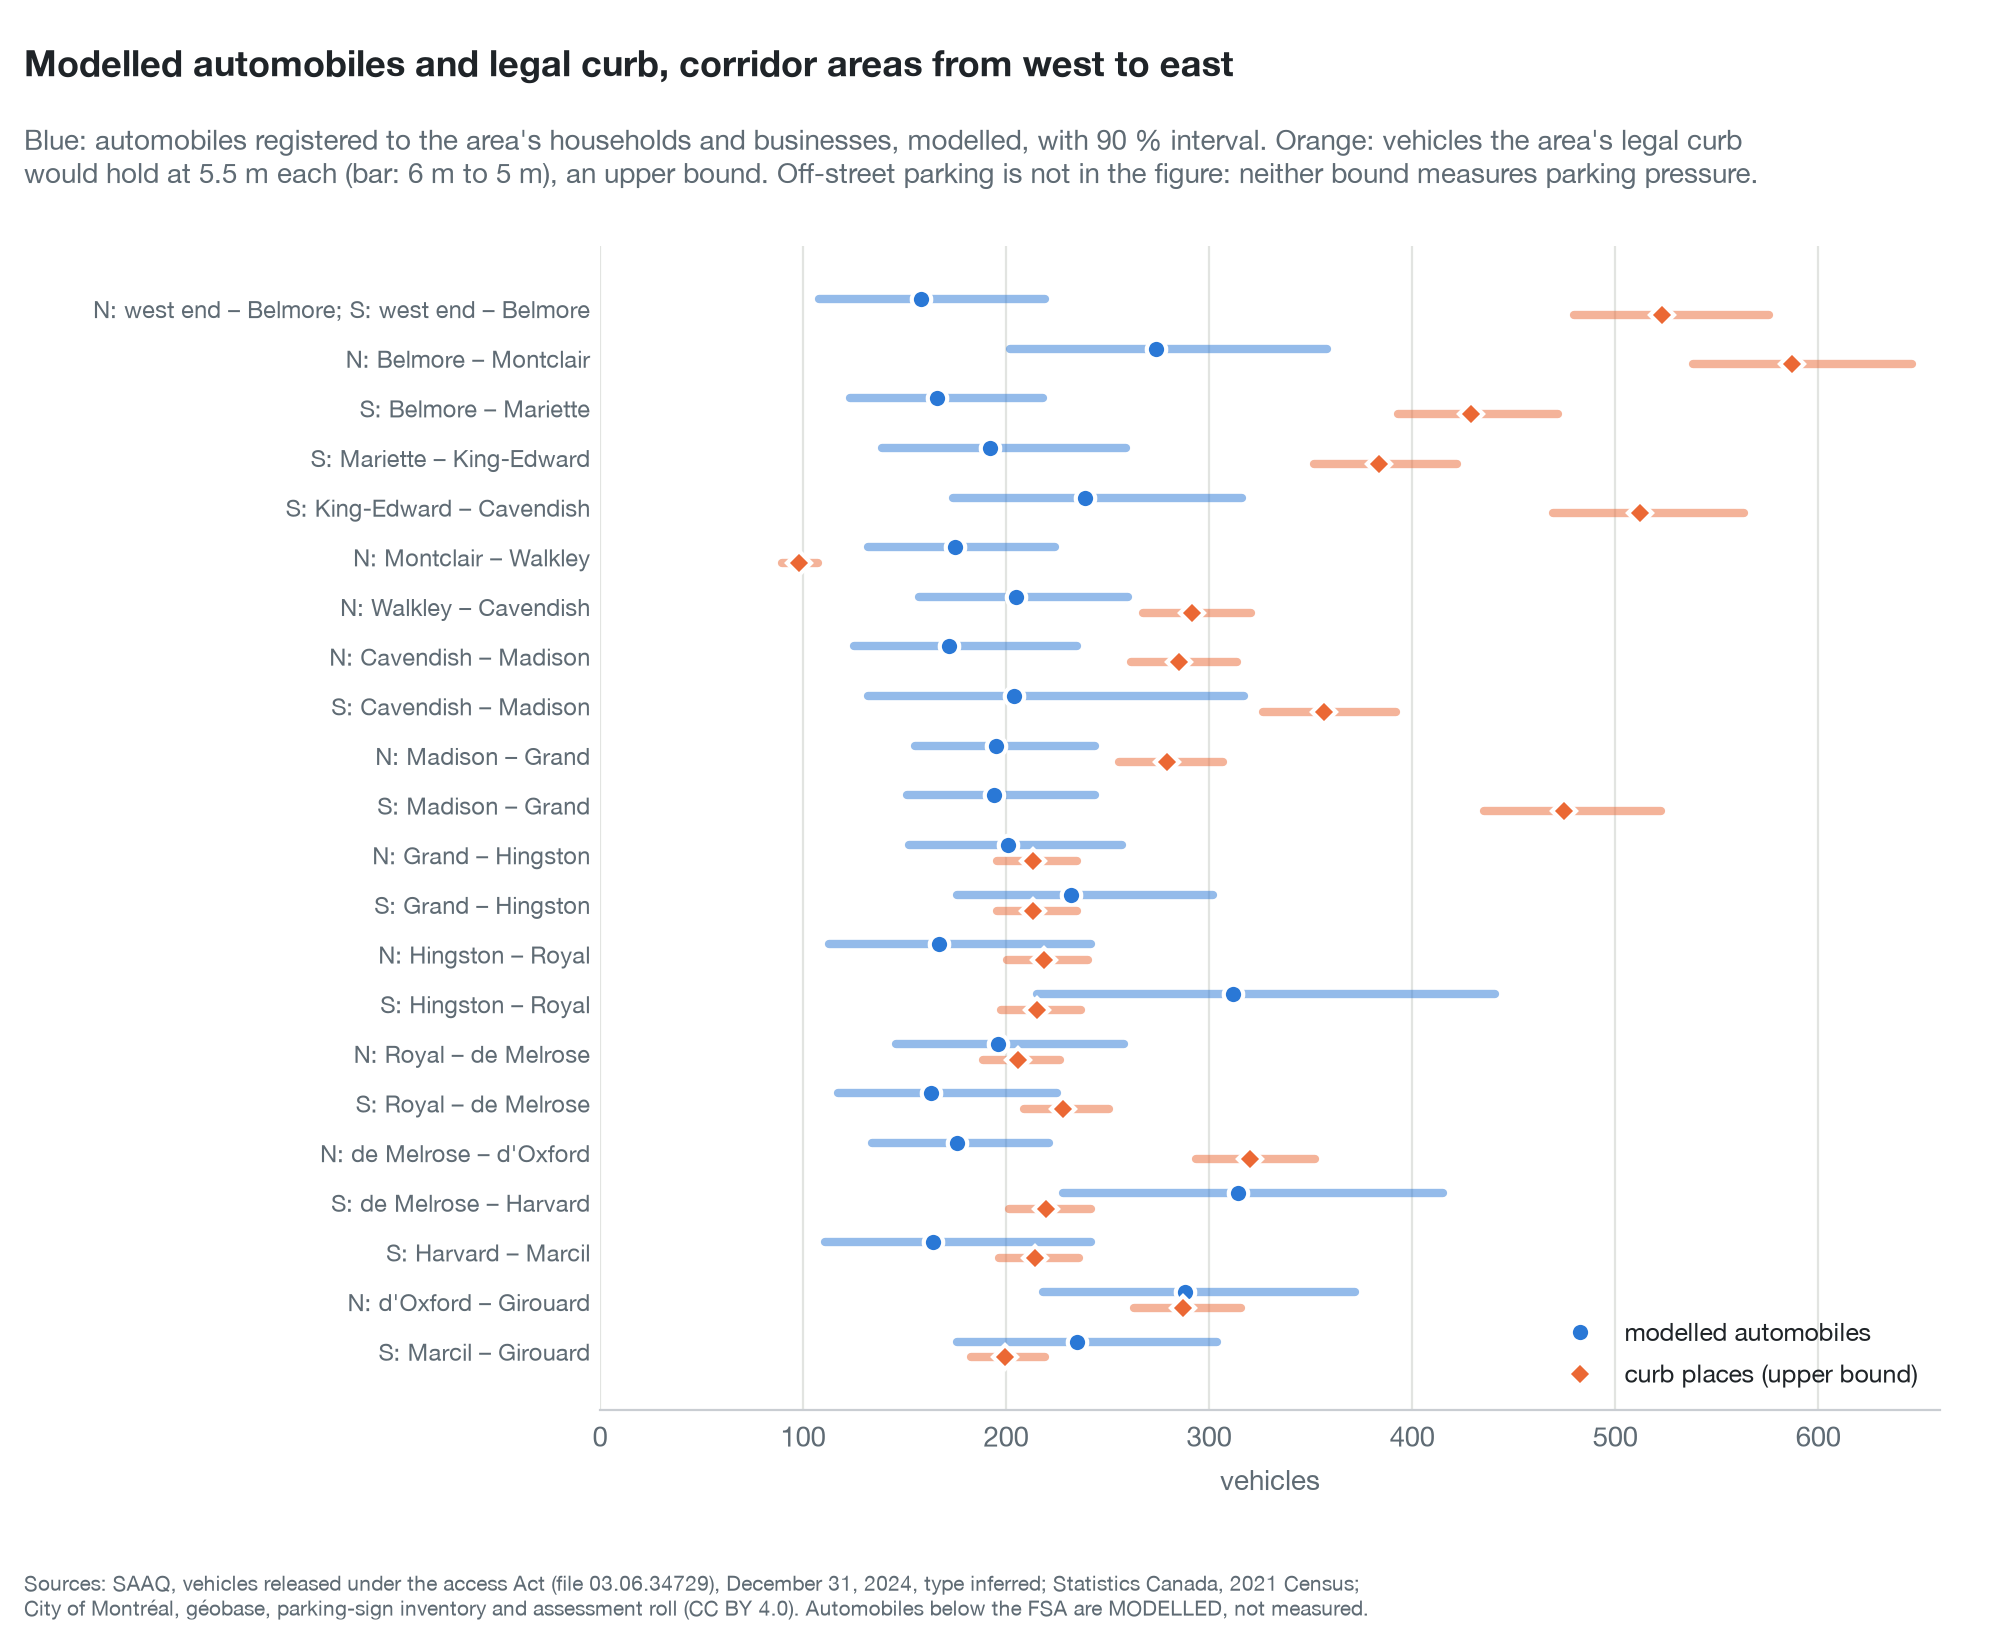
\includegraphics[width=\textwidth]{../derived/figures/curb-and-automobiles/curb_and_automobiles_en.png}\caption{Modelled automobiles and the places the legal curb would hold, by area.}\label{fig:both}\end{figure}

\subsection{A check from the 2015 LiDAR night}
The City\textquoteright{}s 2015 LiDAR was flown at night. Counted by eye along rue de Terrebonne: 183 cars at the curbs and 253 on the lots along the street, 436 for the 573 dwellings addressed on the street: 0.76 per dwelling. The model gives 0.84 per household for the areas that hold those dwellings.
\begin{table}[H]\centering\small
\caption{Cars seen on the 2015 LiDAR night along rue de Terrebonne, and the model, by sector of the 2023 study.}
\begin{tabular}{@{}lrrrrr@{}}\toprule
Sector & dwellings & at curbs & on lots & seen per dwelling & modelled per household \\\midrule
Residential west & 146 & 52 & 97 & 1.02 & 0.93 \\
Institutional & 140 & 29 & 45 & 0.53 & 0.66 \\
Residential east & 287 & 102 & 111 & 0.74 & 0.89 \\
Whole lane & 573 & 183 & 253 & 0.76 & 0.84 \\
\bottomrule\end{tabular}\end{table}
The two quantities are not the same: the LiDAR sees visitors\textquoteright{} cars and the lots of churches, schools and corner buildings addressed on the cross streets, and does not see cars inside garages or away for the night; nine years separate the two. They agree in order of magnitude. They do not agree in detail: across the 11 areas with ten dwellings or more on Terrebonne, the rank correlation between cars seen per dwelling and the modelled rate is 0.31 ($p$ = 0.36), not distinguishable from none. The check therefore supports the level of the estimate, not the split between areas.

\begin{figure}[H]\centering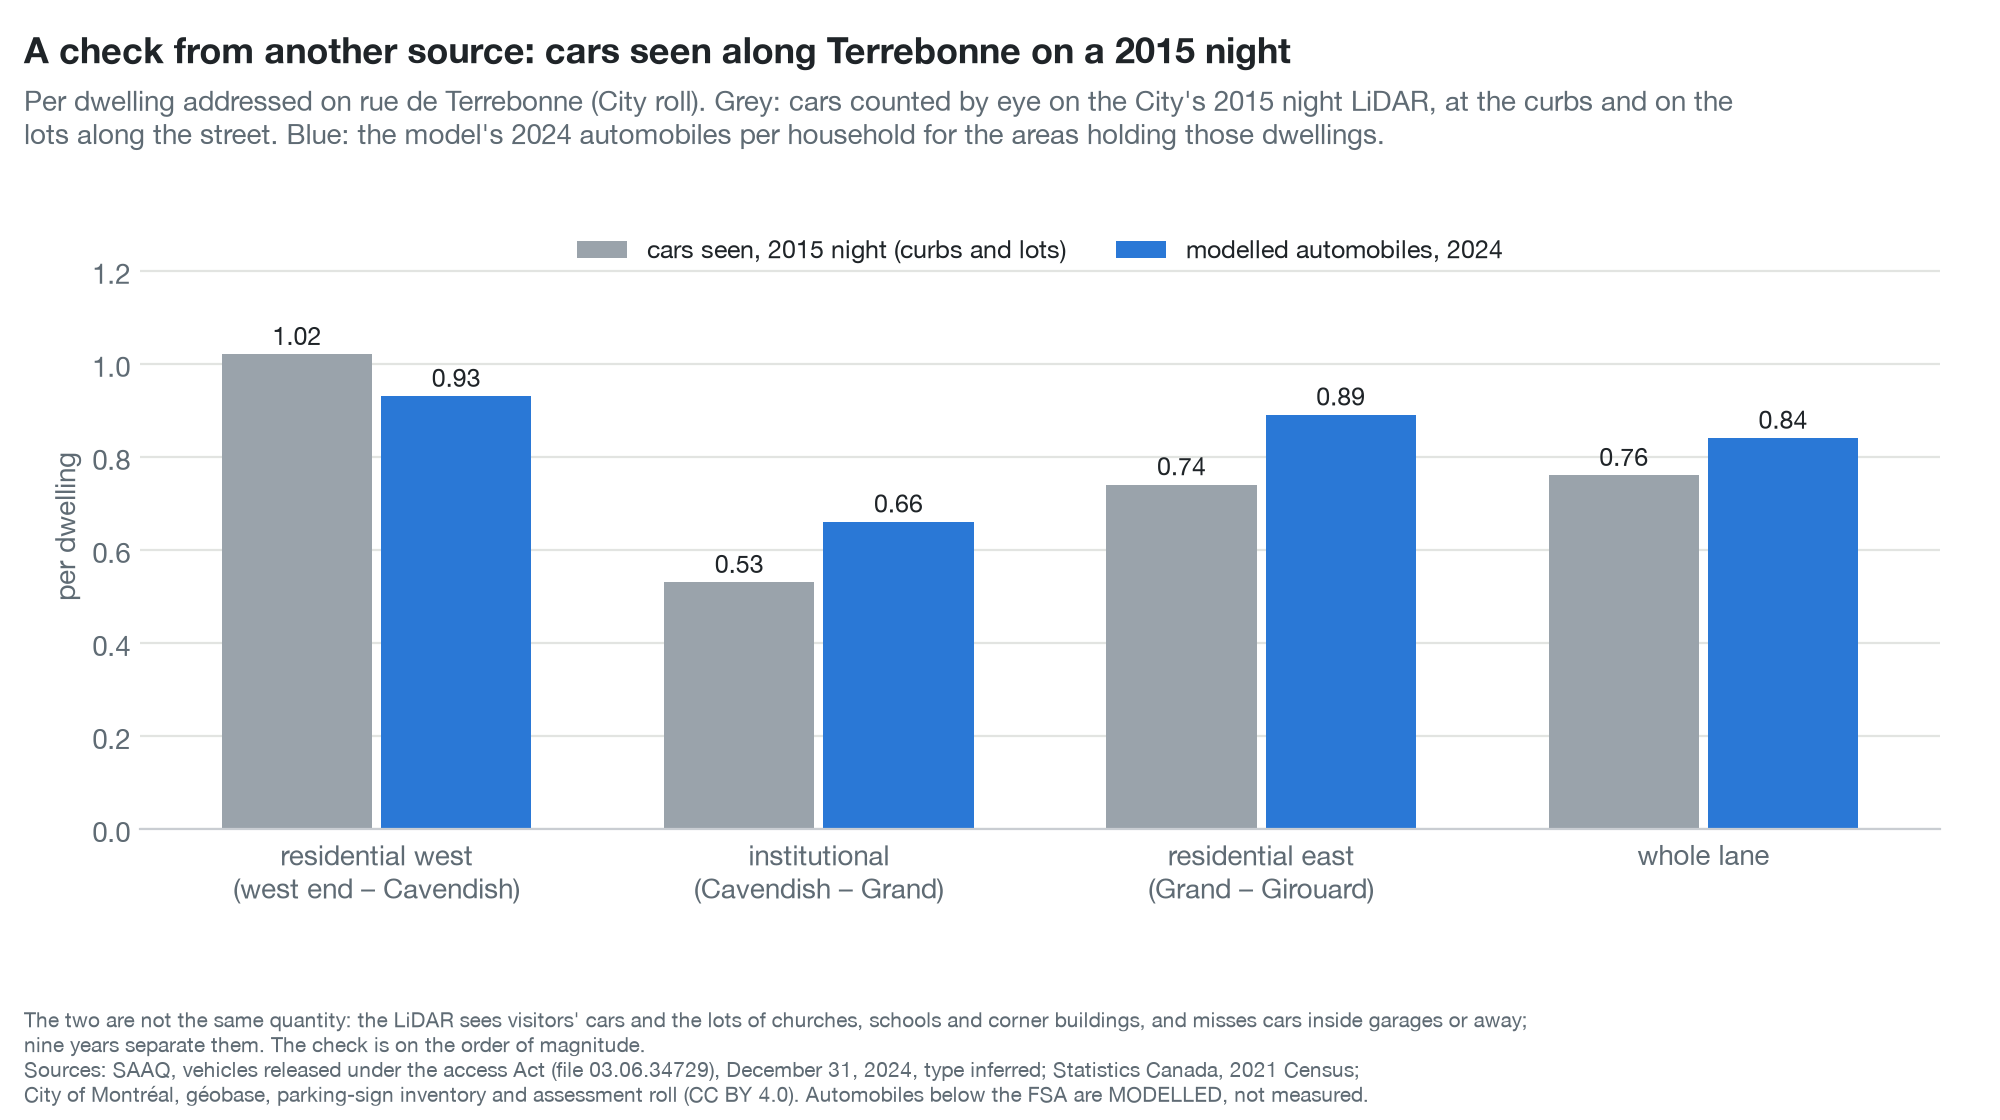
\includegraphics[width=0.9\textwidth]{../derived/figures/lidar-check/lidar_check_en.png}\caption{Cars seen per dwelling on the 2015 night and the model\textquoteright{}s rate, by sector.}\end{figure}

\section{What the note shows and does not show}
\begin{itemize}
\item \textbf{Measured:} the registered automobiles of H4A and H4B (type inferred); the legal curb of each block face, as an upper bound; the dwellings and, on rue de Terrebonne, the garages and driveways.
\item \textbf{Modelled:} the automobiles of every area smaller than an FSA. The model shares a known total better than households alone at the one level where this can be tested; below the FSA nothing can test it, and the 2015 check does not confirm its area-by-area differences.
\item \textbf{Not measured by anyone:} off-street places beyond rue de Terrebonne; where registered vehicles are kept; occupancy of the curb since the lane was built.
\item The curb reading rests on the sign inventory as published on October 23, 2026 and on rules for arrows that were checked on rue de Terrebonne only.
\end{itemize}

\section{Reproducibility}
Scripts, tables and figures: \url{https://github.com/OpenMobilityData/Terrebonne-open-sources/tree/main/2026-terrebonne-corridor-vehicles-and-curb}. Order: \texttt{build\_dataset.py}, \texttt{curb\_supply.py}, \texttt{demand\_model.py}, \texttt{corridor.py}, the figure scripts under \texttt{derived/figures/}, \texttt{build\_docs.py}. The census, roll, sign and postal-code files are read from outside the repository (sources and dates in the folder\textquoteright{}s README); the tables by dissemination area and by block face are in \texttt{derived/tables/}.

\appendix
\section{Tables}
\begin{table}[H]\centering\small
\caption{Specifications compared, each FSA left out in turn: absolute error of the predicted rate (\%), and the signed error for H4A and H4B.}\label{tab:spec}
\begin{tabular}{@{}p{7.4cm}rrrrr@{}}\toprule
Variables & median & 75th & 90th & H4A & H4B \\\midrule
households only & 35.9 & 50.2 & 98.3 & +40.0 & +58.9 \\
tenure, dwelling type & 14.7 & 29.8 & 51.0 & +29.9 & +6.4 \\
commuting & 7.9 & 13.8 & 25.2 & $-$15.3 & +2.4 \\
tenure, commuting, household size & 5.5 & 10.9 & 25.8 & $-$10.8 & +0.2 \\
tenure, commuting, household size, income (used) & 5.4 & 11.0 & 24.4 & $-$10.7 & $-$0.6 \\
tenure, commuting, household size, income, dwelling type & 6.1 & 11.3 & 27.0 & $-$9.9 & $-$2.1 \\
\bottomrule\end{tabular}\end{table}
\begin{table}[H]\centering\small
\caption{Coefficients of the model used (logarithm of automobiles per household; robust regression, 114 FSAs).}
\begin{tabular}{@{}lrr@{}}\toprule
Variable & coefficient & standard error \\\midrule
constant & $-$2.620 & 0.783 \\
share of renter households & +0.015 & 0.114 \\
share of commuters who drive & +2.013 & 0.114 \\
persons per household & +0.198 & 0.047 \\
log of median household income & +0.091 & 0.066 \\
\bottomrule\end{tabular}\end{table}
{\small
\begin{longtable}{@{}p{5.6cm}lrrrrrr@{}}
\caption{The corridor\textquoteright{}s dissemination areas, west to east. N, S: side of rue de Terrebonne and the cross streets the frontage runs between. Automobiles: modelled, with 90\,\% interval. Places: legal curb at 5.5\,m (upper bound).}\label{tab:da}\\\toprule
Frontage on Terrebonne & FSA & hh. & autos & interval & per hh. & curb km & places \\\midrule\endhead
N: west end -- Belmore; S: west end -- Belmore & H4B & 176 & 158 & 108--219 & 0.90 & 2.88 & 523 \\
N: Belmore -- Montclair & H4B & 249 & 274 & 202--358 & 1.10 & 3.23 & 587 \\
S: Belmore -- Mariette & H4B & 273 & 166 & 123--218 & 0.61 & 2.36 & 429 \\
S: Mariette -- King-Edward & H4B & 231 & 192 & 139--259 & 0.83 & 2.11 & 384 \\
S: King-Edward -- Cavendish & H4B & 225 & 239 & 174--316 & 1.06 & 2.82 & 512 \\
N: Montclair -- Walkley & H4B & 208 & 175 & 132--224 & 0.84 & 0.54 & 98 \\
N: Walkley -- Cavendish & H4B & 283 & 205 & 157--260 & 0.72 & 1.60 & 292 \\
N: Cavendish -- Madison & H4V & 233 & 172 & 125--235 & 0.74 & 1.57 & 285 \\
S: Cavendish -- Madison & H4B & 316 & 204 & 132--317 & 0.65 & 1.96 & 356 \\
N: Madison -- Grand & H4B & 260 & 195 & 155--244 & 0.75 & 1.54 & 279 \\
S: Madison -- Grand & H4B & 253 & 194 & 151--244 & 0.77 & 2.61 & 475 \\
N: Grand -- Hingston & H4B & 270 & 201 & 152--257 & 0.74 & 1.17 & 213 \\
S: Grand -- Hingston & H4B & 323 & 232 & 176--302 & 0.72 & 1.17 & 213 \\
N: Hingston -- Royal & H4A & 192 & 167 & 113--242 & 0.87 & 1.20 & 219 \\
S: Hingston -- Royal & H4A & 267 & 312 & 215--441 & 1.17 & 1.18 & 215 \\
N: Royal -- de Melrose & H4A & 204 & 196 & 146--258 & 0.96 & 1.13 & 206 \\
S: Royal -- de Melrose & H4A & 200 & 163 & 117--225 & 0.82 & 1.25 & 228 \\
N: de Melrose -- d'Oxford & H4A & 259 & 176 & 134--221 & 0.68 & 1.76 & 320 \\
S: de Melrose -- Harvard & H4A & 249 & 314 & 228--415 & 1.26 & 1.21 & 220 \\
S: Harvard -- Marcil & H4A & 186 & 164 & 111--242 & 0.88 & 1.18 & 214 \\
N: d'Oxford -- Girouard & H4A & 325 & 288 & 218--372 & 0.89 & 1.58 & 287 \\
S: Marcil -- Girouard & H4A & 289 & 235 & 176--304 & 0.81 & 1.10 & 199 \\
\bottomrule\end{longtable}}
\end{document}
